% **************************************************
% Document Class Definition
% **************************************************
\documentclass[%
    paper=A4,                    % paper size --> A4 is default in Germany
    twoside=true,               % onesite or twoside printing
    openright,                  % doublepage cleaning ends up right side
    parskip=full,               % spacing value / method for paragraphs
    chapterprefix=true,         % prefix for chapter marks
    11pt,                       % font size
    headings=normal,            % size of headings
    bibliography=totoc,         % include bib in toc
    listof=totoc,              % include listof entries in toc
    titlepage=on,              % own page for each title page
    captions=tableabove,        % display table captions above the float env
    draft=false,               % value for draft version
]{scrreprt}%

% **************************************************
% Information and Commands for Reuse
% **************************************************
\newcommand{\thesisTitle}{Business Process Model using Large Language Models}
\newcommand{\thesisName}{Mahdi Ghafarhashemi}
\newcommand{\thesisSubject}{BPMN and LLMs}
\newcommand{\thesisDate}{\today}
\newcommand{\thesisVersion}{Final}


\newcommand{\thesisFirstReviewer}{Prof. Dr.-Ing. Stefan Jablonski}
\newcommand{\thesisFirstReviewerUniversity}{\protect{Universit{\"a}t Bayreuth}}
\newcommand{\thesisFirstReviewerDepartment}{Fakult{\"a}t Mathematik, Physik, Informatik}

\newcommand{\thesisSecondReviewer}{Dr. Sebastian Petter}
\newcommand{\thesisSecondReviewerUniversity}{\protect{Universit{\"a}t Bayreuth}}
\newcommand{\thesisSecondReviewerDepartment}{Fakult{\"a}t Mathematik, Physik, Informatik}

\newcommand{\thesisFirstSupervisor}{Yen Tran}


\newcommand{\thesisUniversity}{\protect{Universit{\"a}t Bayreuth}}
\newcommand{\thesisUniversityDepartment}{Fakult{\"a}t Mathematik, Physik, Informatik}
\newcommand{\thesisUniversityInstitute}{Institut f{\"u}r Informatik}
\newcommand{\thesisUniversityGroup}{Lehrstuhl f{\"u}r Angewandte Informatik IV}
\newcommand{\thesisUniversityCity}{Bayreuth}
\newcommand{\thesisUniversityStreetAddress}{Universit{\"a}tsstrasse 30}
\newcommand{\thesisUniversityPostalCode}{95447}

% **************************************************
% Load and Configure Packages
% **************************************************


\usepackage[utf8]{inputenc}
\usepackage[english]{babel}     % babel system, adjust the language of the content
\usepackage[					% clean thesis style
	figuresep=colon,%
	sansserif=false,%
	hangfigurecaption=false,%
	hangsection=true,%
	hangsubsection=true,%
	colorize=full,%
	colortheme=bluemagenta,%
	bibsys=bibtex,%
	bibfile=bib-refs,%
	bibstyle=alphabetic,
  backref=true%
]{cleanthesis}




\hypersetup{					% setup the hyperref-package options
	pdftitle={\thesisTitle},	% 	- title (PDF meta)
	pdfsubject={\thesisSubject},% 	- subject (PDF meta)
	pdfauthor={\thesisName},	% 	- author (PDF meta)
	plainpages=false,			% 	-
	colorlinks=false,			% 	- colorize links?
	pdfborder={0 0 0},			% 	-
	breaklinks=true,			% 	- allow line break inside links
	bookmarksnumbered=true,		%
	bookmarksopen=true			%
}

%----- edit khodammm
\usepackage{geometry}
\usepackage{amsmath}           % For mathematical typesetting
\usepackage{booktabs}          % For professional tables
\usepackage{multirow}          % For multi-row cells in tables
\usepackage{enumitem}          % For customizing lists
\setlist[itemize]{noitemsep}
\setlist[enumerate]{noitemsep}
\usepackage{algorithm}         % For algorithm environments
\usepackage{algpseudocode}     % For pseudocode formatting
\usepackage{graphicx}          % For including images
\usepackage{float}             % For better table placement
\usepackage{caption}  % For enhanced caption styling
\usepackage{colortbl} % For colored table cells
\usepackage{xcolor}   % For color definitions
\definecolor{lightgray}{gray}{0.9}
\usepackage{pgfplots}
\usepackage{hyperref}





%----- edit khodammm


\graphicspath{ {img/} }


% **************************************************
% Document CONTENT
% **************************************************


\begin{document}
	
	
% --- Title pages: no visible page numbers, roman numbering ---
\pagenumbering{roman}			% roman page numbing (invisible for empty 
\pagestyle{empty}	

% ------------------------------------  --> cover title page
\begin{titlepage}
	\pdfbookmark[0]{Cover}{Cover}
	\includegraphics[width=10cm]{gfx/AI4.png} \\[2mm]
	\flushright
	\vfill
	{\LARGE\thesisTitle \par}
	\rule[5pt]{\textwidth}{.4pt} \par
	{\Large\thesisName}
	\vfill
	\textit{\large\thesisDate} \\
	Version: \thesisVersion
\end{titlepage}

% ------------------------------------  --> cover title page







% ------------------------------------  --> main title page


\begin{titlepage}
	\pdfbookmark[0]{Titlepage}{Titlepage}
	\tgherosfont
	\centering
	
	{\Large \thesisUniversity} \\[4mm]
	\textsf{\thesisUniversityDepartment} \\
	\textsf{\thesisUniversityInstitute} \\
	\textsf{\thesisUniversityGroup} \\
	
	\vfill
	{\large \thesisSubject} \\[5mm]
	{\LARGE \color{ctcolortitle}\textbf{\thesisTitle} \\[10mm]}
	{\Large \thesisName} \\
	
	\vfill
	\begin{minipage}[t]{.27\textwidth}
		\raggedleft
		\textit{1. Reviewer}
	\end{minipage}
	\hspace*{15pt}
	\begin{minipage}[t]{.65\textwidth}
		{\Large \thesisFirstReviewer} \\
		{\small \thesisFirstReviewerDepartment} \\[-1mm]
		{\small \thesisFirstReviewerUniversity}
	\end{minipage} \\[5mm]
	\begin{minipage}[t]{.27\textwidth}
		\raggedleft
		\textit{2. Reviewer}
	\end{minipage}
	\hspace*{15pt}
	\begin{minipage}[t]{.65\textwidth}
		{\Large \thesisSecondReviewer} \\
		{\small \thesisSecondReviewerDepartment} \\[-1mm]
		{\small \thesisSecondReviewerUniversity}
	\end{minipage} \\[10mm]
	\begin{minipage}[t]{.27\textwidth}
		\raggedleft
		\textit{Supervisor}
	\end{minipage}
	\hspace*{15pt}
	\begin{minipage}[t]{.65\textwidth}
		\thesisFirstSupervisor
	\end{minipage} \\[10mm]
	
	\thesisDate \\
	
\end{titlepage}


% ------------------------------------  --> lower title back for single page layout
\hfill
\vfill
{
	\small
	\textbf{\thesisName} \\
	\textit{\thesisTitle} \\
	\thesisSubject, \thesisDate \\
	Reviewers: \thesisFirstReviewer\ and \thesisSecondReviewer \\
	Supervisor: \thesisFirstSupervisor\\[1.5em]
	\textbf{\thesisUniversity} \\
	\textit{\thesisUniversityGroup} \\
	\thesisUniversityInstitute \\
	\thesisUniversityDepartment \\
	\thesisUniversityStreetAddress \\
	\thesisUniversityPostalCode\ \thesisUniversityCity\\ Germany
}



% --- End of title pages, start showing roman numbers ---
\cleardoublepage

\pagestyle{plain}				% display just page numbers

% --- Table of contents and other front matter ---
\setcounter{tocdepth}{3}
\tableofcontents
%


\cleardoublepage

% --- Main content, switch to arabic numbers ---
\pagenumbering{arabic}
\setcounter{page}{1}
\pagestyle{plain}





\chapter{Introduction}


\cleanchapterquote{The future of Artifical Intelligence is not about replacing humans, it's about augmenting human capabilities.}{Sundar Pichai}{CEO of Google}

Recent advances in Large Language Models (LLMs) have stimulated extensive research into their various applications. One particularly promising domain is their use for Business Process (BP) comprehension. A vital aspect of any organization lies in the ability to make well-informed decisions based on available data and resources, a role traditionally fulfilled by Decision Support Systems (DSS), which may involve human experts or software solutions. LLMs present a novel opportunity to enhance or even assume this role by harnessing their robust natural language understanding and generation capabilities.

However, BP modeling presents several challenges, including comprehending process structures, interpreting their attributes, and accessing all pertinent enterprise content. Although some studies have explored the integration of LLMs into such systems, new concerns have arisen, particularly regarding the factual reliability of the information these models provide.

The primary focus of this study is to address three key questions: How can LLMs be augmented and utilized to extract BP knowledge? What are the potential and key challenges associated with fine-tuning and the Retrieval-Augmented Generation (RAG) method? How can the performance of such systems be effectively evaluated?

The central objective is the development of process-aware conversational Decision Support Systems using LLMs within the context of BP, drawing insights from two papers by \cite{franzoi2024using} and \cite{bernardi2024conversing}.

The paper is organized as follows: \textbf{Chapter~\ref{Background}} provides background information and introduces the core concepts behind the methods and techniques implemented in both papers. \textbf{Chapter~\ref{related work}} reviews related work on the main topic. \textbf{Chapter~\ref{processknowledge}} explores how process knowledge can be extracted from BPs using diverse approaches. One approach features a prototype implementation of an LLM-based chatbot capable of identifying process knowledge across various forms of enterprise content, irrespective of specific representations. The other approach examines the Business Process Large Language Model (BPLLM) framework, which integrates RAG with fine-tuning.\textbf{Chapter~\ref{challenges}} discusses the challenges encountered during implementation, as well as additional limitations observed in practice. \textbf{Chapter~\ref{evaluation}} presents methods for evaluating the performance of such systems and elucidates the evaluation strategies employed by the authors in their respective approaches. Finally, \textbf{Chapter~\ref{conclusion}} offers a conclusion on the topic.



\chapter{Background}
\section{Business Process Model}
\label{Background}



A business process model is a graphical representation of a BP or workflow and its related subprocesses \cite{hammer2014business}. Process modeling produces activity diagrams and flowcharts that provide critical insights into the operation of a particular process, including:
\begin{itemize}
	\item Events and activities that occur within the workflow.
	\item The individuals or roles responsible for initiating these events and activities.
	\item Decision points and the alternative paths a workflow can follow depending on the outcomes.
	\item Timelines of the overall process as well as each individual step.
\end{itemize}



\textbf{Business Process Model and Notation}\hspace{0.5em}
Business Process Model and Notation (BPMN) is a standardized graphical notation for modeling BPs, providing visual representations of their components and semantics. It is designed to be useful for both technical users and business stakeholders \cite{omg2013bpmn}.




\section{Large Language Models }
LLMs are transformer-based language models that contain hundreds of billions (or more) of parameters and are trained on massive text corpora. These models, such as GPT-4 \cite{achiam2023gpt} and LLaMA \cite{touvron2023llama}, are capable of understanding and generating natural language, and can perform a wide range of tasks.

\section{Parameter-Efficient Fine-Tuning}

Events, facts, and recent information after the model's training cutoff date are not known to the model unless it is fine-tuned or updated.  
The advent of LLMs has reshaped natural language processing, revealing that pre-trained language models (PLMs) \cite{devlin2019bert} alone frequently cannot fulfill specialized demands. To address this, researchers \cite{howard2018universal} introduced the concept of \textit{fine-tuning}, in which the parameters of a pre-trained model are updated using a task-specific dataset with labelled answers.
However, modern LLMs contain billions of parameters, and fully fine-tuning all of them is computationally expensive, memory-intensive, and often prone to overfitting, especially when training data is limited. To overcome these limitations, a more efficient approach known as Parameter-Efficient Fine-Tuning (PEFT) has been proposed \cite{xu2023parameter}.
PEFT updates only a small subset of the model's parameters while keeping the majority frozen. Several methods fall under the PEFT framework, including Low-Rank Adaptation (LoRA) \cite{hu2022lora} and Prompt Tuning, each offering distinct trade-offs between efficiency and flexibility.


\section{Quantization}

Quantization is a technique used to reduce the size and increase the speed of LLMs \cite{wu2020integer}.In these models, numerical values are typically stored as 32-bit floating-point numbers (float32). Quantization reduces the precision of these values by using fewer bits, such as 8-bit integers (int8) or even 4-bit integers (int4). However, this comes with a trade-off: while quantization saves memory and improves performance, it may slightly reduce the model's accuracy due to the use of less precise representations.


\section{Retrieval-Augmented Generation }

With the emergence of LLMs, several challenges have arisen, including \textit{hallucination} \cite{marcus2020next}, poor performance on domain-specific tasks, and, most notably, the lack of long-term memory,particularly critical in conversational settings. To address these limitations, hybrid models \cite{guu2020retrieval} have been introduced that combine parametric memory and non-parametric memory.
Parametric memory refers to knowledge encoded within the model’s internal parameters during pretraining. In contrast,non-parametric memory involves mechanisms that allow the model to access external data sources,such as  a document corpora or databases at inference time. A key limitation of purely parametric models is that their internal knowledge cannot be updated dynamically; updates require costly retraining or fine-tuning. RAG \cite{lewis2020retrieval} addresses this by integrating both types of memory, enabling models to incorporate external, updatable knowledge while still leveraging their internally learned representations.

RAG is formulated as a probabilistic framework comprising two main components: a retriever and a generator \cite{lewis2020retrieval}.

\subsection{Retriever}

The effectiveness of RAG largely depends on the quality of the retrieved documents. Consequently, various retrieval mechanisms have been proposed depending on the use case, many of which rely on similarity-based approaches.
After retrieval, RAG systems use cross-attention mechanisms that allow the model to focus on the retrieved context. When integrating this information into the generative component, it is crucial that the most relevant retrieved content is emphasized and not lost during the generation phase.




\textbf{Mechanism of Retrieval}\hspace{0.5em}One traditional method is BM25 \cite{robertson2009probabilistic}, which calculates the relevance score of a document with respect to a user's query based on the frequency of query terms within the document. Due to its simplicity and efficiency, BM25 is well-suited for keyword-matching scenarios and remains widely used in various applications.

Another widely used approach is Dense Passage Retrieval (DPR), introduced by \cite{karpukhin2020dense}. This method enables efficient k-nearest-neighbor search \cite{xiong2020approximate}. Unlike BM25, DPR captures the semantic meaning of text by embedding passages and queries into a shared vector space \cite{gupta2024comprehensive}. This approach is particularly effective for open-domain question-answering tasks. Recent research \cite{li2023making} demonstrates that DPR, when combined with pre-trained language models, can outperform BM25 in retrieval accuracy.


The following section focuses on a retrieval component based on DPR \cite{lewis2020retrieval}.

Given an input \( x \) (e.g., a query or document), the retriever returns the top-\( K \) most relevant passages from a large corpus by modeling a probability distribution over all candidate documents as:

\[
p_{\eta}(z \mid x)
\]

where \( p_{\eta} \) is the retriever parameterized by \( \eta \), and \( z \) is a retrieved passage.

The retriever uses a bi-encoder architecture comprising two independent BERT-based encoders \cite{devlin-etal-2019-bert}: one for the query \( x \) and one for the documents \( z \). The document encoder computes a dense representation:

\[
d(z) = \text{BERT}_{\text{doc}}(z)
\]

The query encoder computes:

\[
q(x) = \text{BERT}_{\text{query}}(x)
\]

Each encoder independently maps its input into a vector in a shared embedding space.

To measure the relevance between a document \( z \) and the query \( x \), the dot product of their embeddings is computed:

\[
\text{score}(z, x) = d(z)^\top \cdot q(x)
\]

This score ranks the top-\( K \) most relevant documents. Since the retrieval model must output a probability distribution, a softmax function is applied over all candidate documents:

\[
p_\eta(z \mid x) \propto \exp\left(d(z)^\top \cdot q(x)\right)
\]

Thus, a higher dot product between the query and document embeddings results in a higher retrieval probability.

To enable efficient search, all documents are pre-encoded using the document encoder:

\[
d(z) = \text{BERT}_{\text{doc}}(z)
\]

These vectors are stored in a vector database. At inference time, the query vector \( q(x) \) is computed and compared against the document index to retrieve the top-\( K \) most relevant passages.





\subsection{Generator}

The second core component of RAG is the generator, which plays an essential role in synthesizing the retrieved information into a contextually appropriate response.The following section describes the generation process using BART (Bidirectional and Auto-Regressive Transformer) model\cite{lewis-etal-2020-bart}.

The generator models the probability of generating the next token given the input, retrieved document, and previously generated tokens:

\[
p_{\theta}(y_i \mid x, z, y_{1:i-1})
\]

This represents the parametric memory of the model, as it relies on the parameters \( \theta \). The generator is typically a pretrained sequence-to-sequence transformer model, which takes an input sequence and produces an output sequence.

The generator produces each output token \( y_i \) based on:
\begin{itemize}
	\item the original input \( x \),
	\item the retrieved document \( z \), and
	\item the previously generated tokens \( y_{1:i-1} \).
\end{itemize}

To integrate both components , retriever and generator , the model marginalizes over the top-\( K \) retrieved documents for each token, combining their probabilities as follows:

\[
p(y \mid x) \approx \prod_{i=1}^{N} \sum_{z \in \text{top-}K(p(\cdot \mid x))} p_\eta(z \mid x) \cdot p_\theta(y_i \mid x, z, y_{1:i-1})
\]

This equation defines the RAG-Token model, where each output token is generated by marginalizing over the probability contributions from multiple documents.


\subsection*{RAG-Token Model}

There are two main variants of RAG models based on \cite{lewis2020}: RAG-Sequence and RAG-Token. In this work, we focus on the RAG-Token model.
Unlike RAG-Sequence,which conditions on a single retrieved document to generate the entire output sequence.RAG-Token allows the model to condition on different retrieved documents at each token position. This enables the generator to dynamically select the most relevant content from various documents while generating each word of the output.

The final probability of the entire output sequence is given by:

\[
p_{\text{RAG-Token}}(y \mid x) \approx \prod_{i=1}^{N} \sum_{z \in \text{top-}K(p(\cdot \mid x))} p_\eta(z \mid x) \cdot p_\theta(y_i \mid x, z, y_{1:i-1})
\]

This approach provides greater flexibility by allowing different retrieved documents to influence different parts of the generated output, which is especially useful for complex, multi-faceted questions.




\section{Chatbot Evaluation Framework}

With the growing popularity of chatbots, it is evident that appropriate metrics are needed to evaluate their outputs. However, there is currently no unified standard for assessing chatbot performance. One possible solution to this challenge is to align evaluation metrics with different perspectives of chatbot assessment \cite{peras2018chatbot}. These perspectives include the user experience perspective, information retrieval perspective, linguistic perspective, technology perspective, and business perspective.To construct a comprehensive evaluation framework, the following categories should be considered and analyzed: usability, performance, affect, satisfaction, accuracy,accessibility, efficiency, quality, quantity, relation, manner, grammatical accuracy, humanity, and business value.

\chapter{Related work}


\label{related_work}

Business process knowledge extraction using RAG and fine-tuned LLMs facilitates structured insights from unstructured data. Recent work in this field typically focuses on domain-specific applications or structured knowledge extraction.

\citet{chen2025application} introduce an Interactive Industrial Knowledge Management (IIKM) system that applies RAG to extract information from technical manuals and regulatory documents, including human resource policies. Similarly, \citet{bahr2025knowledge} integrate knowledge graphs into RAG pipelines to perform Failure Mode and Effects Analysis (FMEA), enabling insight extraction from industrial documentation. In parallel, \citet{efeoglu2024retrieval} propose a relation extraction framework combining RAG and fine-tuned LLMs to identify entities such as roles and tasks from process descriptions. These approaches structure extract knowledge into machine-interpretable formats using knowledge graphs, supporting downstream applications such as automation and risk analysis.

A common trend across these studies is the use of hybrid retrieval strategies that combine sparse (e.g., BM25) and dense search, to improve relevance \citep{chen2025application}. Domain-specific fine-tuning of LLMs further boosts accuracy \citep{chen2025application, efeoglu2024retrieval, bahr2025knowledge}. The integration of knowledge graphs remains central, enabling structured representations for compliance checks, risk assessment, and workflow optimization.

The state of the art emphasizes combining robust retrieval, domain adaptation, and graph-based structuring. \citet{chen2025application} improve retrieval precision, while \citet{bahr2025knowledge} apply structured outputs for early risk detection. \citet{efeoglu2024retrieval} validate generalizability using benchmarks. Evaluation commonly targets relevance and extraction fidelity.

Nonetheless, challenges persist. Scalability to large datasets and real-time systems remains difficult \citep{chen2025application}. Limited multilingual capabilities reduce global usability \citep{efeoglu2024retrieval}, and heavy domain-specific tuning limits cross-domain flexibility \citep{bahr2025knowledge}. Moreover, process-specific evaluation metrics and privacy-preserving approaches are still underdeveloped. These gaps highlight the need for scalable, domain-agnostic frameworks with tailored evaluation and stronger privacy controls.












\chapter{Process knowledge extraction}
\label{processknowledge}

Process knowledge can exist in various data formats, such as videos, slides, photos, process models, and more, and may be dispersed across different parts of an enterprise. Accessing and integrating all of this information to construct a comprehensive process model can be challenging.

\section{First approach: Low-Code-Based Framework}

The first approach \cite{franzoi2024using} presents a prototype that features an LLM-based chatbot capable of retrieving process knowledge from both structured and unstructured enterprise content. It answers user queries based upon domain-specific training data.
To implement this prototype, the authors \cite{franzoi2024using} use Flowise - a low-code platform that enables non-programmers to easily develop and connect components for LLM applications. By adopting RAG, the process becomes more efficient and manageable.
To reduce hallucination, the authors also implement mechanisms to guide the model’s behavior in cases where the required information is not available.


\begin{figure}[h]
	\centering
	\includegraphics[scale=0.1]{Blank_diagram}
	\caption{Architecture of the Prototype, adapted from \cite{franzoi2024using}.}
	\label{fig:Architecture of the Prototype}
\end{figure}

The prototype consists of two main parts:




\subsection{Data Preprocessing}

In this phase, data is extracted from heterogeneous sources, such as presentation slides and BPMN models,using Python scripts. The extracted data is then transformed into a uniform text format.
Subsequently, the authors apply the RecursiveCharacterTextSplitter\footnote{\url{https://python.langchain.com/docs/how_to/recursive_text_splitter/}} to divide the text into manageable chunks. These chunks are then embedded using the OpenAI API and stored in a single vector database, Pinecone\footnote{\url{https://www.pinecone.io/}}.


\subsection{Conversational Retrieval Question Answering Chain}

This component includes a conversational retrieval question answering (QA) chain\footnote{\url{https://flowiseai.com/}}, which enables question answering by combining a retrieval component with similarity search using cosine similarity. The chain acts as a wrapper around OpenAI’s LLM and uses the ChatOpenAI building block to integrate GPT-4\footnote{\url{https://openai.com/index/gpt-4/}} into the overall flow of the prototype. This integration allows the system to store conversational history and generate contextually appropriate responses.

Additionally, the chain leverages OpenAI’s chat endpoint to support explainability \cite{ramchurn2021trustworthy} by linking the sources of the retrieved documents or text used in the response. After fetching data from the retrieval component and preparing a prompt based on the user query, the prompt is passed to the generative model, which produces the final answer.


\section{Second Approach: Code-Based Framework}

The second approach involves implementing a more code-intensive framework, with the core objective of helping users understand BPs, such as activities or sequence flows within a BP model.
To achieve this, the authors \cite{bernardi2024conversing} develop a pipeline that integrates a RAG system with fine-tuning in order to provide more grounded and contextually accurate responses based on the BP model and user queries.
In this implementation, the authors use LangChain\footnote{\url{https://www.langchain.com/}} to construct the pipeline. The external knowledge source in this study consists of BPMN files used as input.
\begin{figure}[h!]
	\centering
	\includegraphics[scale=0.2]{approach2}
	\caption{Architecture of BPLLM}
	\label{app}
\end{figure}

This pipeline is composed of four layers:


\subsection{LLM Fine-Tuning}

For fine-tuning, the authors use the LLaMA 3.1 8B model \cite{touvron2023llama} on a supervised dataset\footnote{\url{https://github.com/huggingface/autotrain-advanced}} based on a specific BP model. The dataset consists of binary questions split into two types:
The first type covers structural information (e.g., which elements, tasks, events, and gateways are present in the process model), while the second type focuses on behavioral information—that is, how these elements interact and connect within the model.

\subsection{Knowledge Augmentation}

\textbf{BPMN-Specific Chunking}\hspace{0.5em}The authors evaluate several chunking methods, including recursive, fixed-size, and BPMN-specific chunking. The best configuration is achieved using BPMN-specific chunking with BPMN files as input, as shown in Table~2 \cite{bernardi2024conversing}. Each chunk consists of 32 tokens with an overlap of 10.

The pipeline begins by reading a BPMN file, typically an XML-based representation of a BP model. It identifies semantically meaningful chunks among core BPMN components such as tasks, events, and gateways, while ignoring graphical elements irrelevant to semantic understanding.

The chunking processor parses the BPMN file by splitting it at relevant XML tags, including \texttt{<task>}, \texttt{<event>}, and \texttt{<gateway>}. Each resulting chunk represents a self-contained unit of process logic that can be understood independently.


\begin{figure}[h]
	\centering

	\includegraphics[scale=0.3]{chunking}
	\caption{Example figure showing BPMN- Specific chunking process, adapted from \cite{bernardi2024conversing}.}
	\label{fig:chunking}
\end{figure}



\textbf{Embedding}\hspace{0.5em}In the embedding phase, each BPMN chunk is transformed into a dense, low-dimensional vector, which is crucial for enabling efficient semantic search and retrieval.
To generate these embeddings, the authors evaluate several pre-trained models. The best-performing model is \texttt{all-MiniLM-L6-v2} \cite{allMiniLM2025}, a compact sentence transformer that maps sentences into dense vector representations within a shared embedding space.

\textbf{Storing}\hspace{0.5em}After the embedding step, the resulting vectors are stored in the Qdrant vector database\footnote{\url{https://qdrant.tech/}}.

\subsection{Retrieval}

LangChain plays a central role in this layer by connecting the retrieval component to the vector database. The authors use the gRPC\footnote{\url{https://grpc.io/docs/what-is-grpc/introduction/}} communication protocol, which is well suited for handling vector similarity searches based on cosine similarity.

Similar to the first approach, this system performs QA tasks by retrieving documents relevant to the user's query. It also supports long-term memory capabilities by preserving interaction history and enhancing context awareness. This retrieval process ensures that the most semantically relevant chunks are surfaced and passed to the generative model for response generation.






  
    


    \chapter{Challenges}
    \label{challenges}
    
   
   The challenges associated with fine-tuning and the RAG method in both presented approaches can be understood by examining the individual components that make up the overall framework. Each component offers opportunities for optimization, whether through advanced techniques, alternative tools, or predefined configurations \cite{gupta2024comprehensive, bernardi2024conversing, franzoi2024using}.
    
    
    \section{Technical}
    
     \textbf{Implemented Framework}\hspace{0.5em}
    As shown in the first approach, the authors adopt a low-code-based framework to simplify implementation and enhance usability for a broad range of users within a company. However, certain scenarios may require more specific configurations that necessitate a code-intensive platform. In such cases, the second approach is more appropriate.
    Ultimately, the choice of framework depends on the business context and the types of users involved. In particular, it may be necessary to tailor the platform to different user groups in order to improve usability and accessibility.
    

    
   \textbf{Input/Output Format}\hspace{0.5em}
   To address the limitations related to the first approach, we begin with the input format. One primary challenge lies in locating or accessing process knowledge within an organization, as such information is often scattered across various sources.
   The second limitation, following the identification of relevant content, pertains to processing the input files. While semi-structured data such as XML files are relatively easy to handle, unstructured data—including audio, voice recordings, or graphical objects—poses significant challenges. Although the first approach is capable of processing various formats of process knowledge, graphical elements may be lost during recursive chunking \cite{franzoi2024using}.
   
   In comparison, the second approach uses structured inputs, such as BP models presented in BPMN files or Directly-Follows Graphs (DFGs) \cite{VANDERAALST2019321}, along with natural language descriptions of BPs (referred to as "Natural Text" in this work). However, it does not support other input formats like presentation slides, videos, or audio files, which could also serve as valuable sources of process knowledge.
   
   A further challenge common to both approaches concerns the output format. In both cases, the output is generated in natural language form. While this is sufficient in many scenarios, there are cases where outputs in other formats—such as video—could improve user understanding of BPs.
   Thus, both input and output representation formats play a critical role in the effectiveness of these systems. Addressing this limitation may require the integration of multimodal RAG systems \cite{yu2024visrag} capable of handling diverse input and output modalities.
  
    
   \textbf{Chunking}\hspace{0.5em}
   One potential reason for using chunking is the limitation of input size for LLMs; it is not possible to provide a large amount of data to an LLM at once.
   Chunking is one of the most important components of a RAG system. If it does not work properly, it can mislead the embedding model. Therefore, several factors must be taken into account:
     \begin{table}[H]
   	\centering
   	\begin{tabular}{|c|c|c|c| c|}
   		\hline
   		\rowcolor{blue!30}
   		Process Model & Chunking & Prompts & Language Model & Accuracy \\
   		\hline
   		Natural Text & - \textsuperscript{†}& - & Llama2 13B \textsuperscript{†} & \cellcolor{yellow!30}65.48\% \\
   		Natural Text & - & Refined 	 & Llama2 13B & 67.27\% \\
   		Natural Text & Fixed & - & Llama2 13B & 54.76\% \\
   		Natural Text & Fixed & Refined & Llama2 13B & 60.71\% \\
   		Natural Text & Recursive  \textsuperscript{†}& - & Llama2 13B &\cellcolor{yellow!30} 55.95\% \\
   		Natural Text & Recursive & Refined & Llama2 13B & 61.90\% \\
   		BPMN & - & - & Llama2 13B & 60.57\% \\
   		BPMN & - & Refined & Llama2 13B & 64.86\% \\
   		BPMN & Fixed & - & Llama2 13B & 60.78\% \\
   		BPMN & Fixed & Refined & Llama2 13B & 73.53\% \\
   		BPMN & Recursive & - & Llama2 13B & 67.65\% \\
   		BPMN & Recursive & Refined & Llama2 13B & 73.53\% \\
   		BPMN & BPMN-specific & Refined & Llama2 7B\textsuperscript{{\hypertarget{model}{*}}} & 68.47\% \\
   		BPMN & BPMN-specific & Refined & Llama 3 8B Instruct \textsuperscript{*} & 89.78\% \\
   		
   		BPMN & BPMN-specific & Refined  \textsuperscript{**}&  Llama 3.1 8B Instruct  & 90.38\% \\
   		\bottomrule
   	\end{tabular}
   	
   	\caption{Evaluation results based on chunking adapted from \cite{bernardi2024conversing}}
   	\label{chunking_table} % Label moved after caption
   	
   	\begin{minipage}{0.9\textwidth}
   		\footnotesize
   		\textsuperscript{*} Switching to a larger Model. \\
   		\textsuperscript{†} As shown, in some cases, the input is small enough that omitting chunking results in better accuracy.\\
   		\textsuperscript{**} Including predefined prompting can improve performance by helping the chunking process achieve higher accuracy.
   		
   		
   	\end{minipage}
   \end{table}
   The first aspect is choosing the LLM responsible for chunking. In the second approach, several models are considered. Based on the inverse scaling phenomenon \cite{mckenzie2023inverse}, it is not always the case that larger models yield better performance. However, as shown in Table~\ref{chunking_table}, switching to a larger model results in improved accuracy.
   The second aspect is selecting the appropriate chunking method, which depends on the size of the input. As shown in Table~\ref{chunking_table}, it can be observed that, based on the type of input—whether natural text or BPMN—a suitable chunking method can be applied. In some cases, the input is small enough to fit into a single chunk, making chunking unnecessary.
   



    
    
    

\textbf{Embedding Models}\hspace{0.5em}
Based on the second approach, it becomes evident that the selection of the embedding model is contingent upon the type of input. Two critical cases merit attention:

The first case involves the significance of model size. For instance, it is observed that an embedding model mapping to a significantly higher-dimensional dense vector does not invariably enhance accuracy (see Figure~\ref{embedding_char}). This outcome depends on the input type or the complexity of the documents, where, in some instances, such models may lead to overfitting.
The second—and arguably more crucial—finding is illustrated in Figure~\ref{embedding_chart}: there are scenarios where the selected embedding model underperforms with chunking due to a critical misalignment between chunking and embedding. When the model is tailored to the input type, the embedding process becomes more effective, thereby boosting accuracy.

\begin{figure}[H]
	\centering
	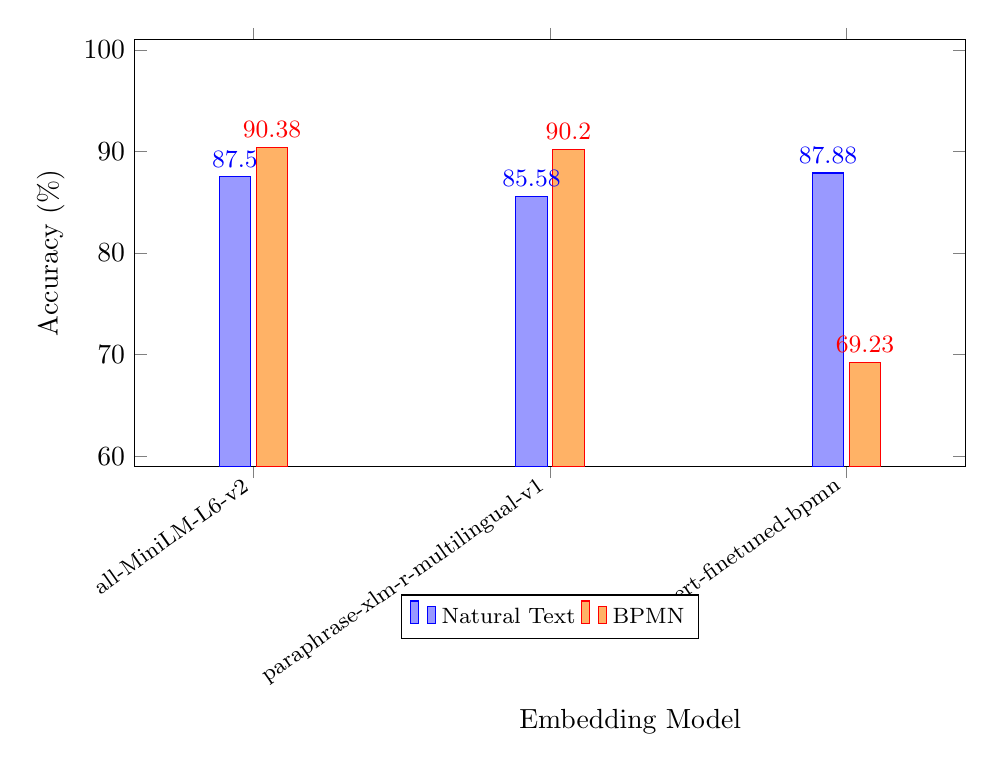
\begin{tikzpicture}
		\begin{axis}[
			ybar,
			bar width=0.4cm,
			enlargelimits=0.2,
			ylabel={Accuracy (\%)},
			xlabel={Embedding Model},
			xlabel style={xshift=2.9em},
			symbolic x coords={all-MiniLM-L6-v2, paraphrase-xlm-r-multilingual-v1, bert-finetuned-bpmn},
			xtick=data,
			xticklabel style={rotate=35, anchor=east, font=\footnotesize},
			nodes near coords,
			nodes near coords align={vertical},
			nodes near coords style={font=\small, yshift=0cm},
			ymin=65, ymax=95,
			legend style={at={(0.5,-0.3)}, anchor=north, legend columns=2, font=\footnotesize},
			width=\textwidth,
			height=7cm
			]
			\addplot+[ybar, fill=blue!40] 
			coordinates {
				(all-MiniLM-L6-v2, 87.50)
				(paraphrase-xlm-r-multilingual-v1, 85.58)
				(bert-finetuned-bpmn, 87.88)
			};
			\addlegendentry{Natural Text}
			
			\addplot+[ybar, fill=orange!60] 
			coordinates {
				(all-MiniLM-L6-v2, 90.38)
				(paraphrase-xlm-r-multilingual-v1, 90.20)
				(bert-finetuned-bpmn, 69.23)
			};
			\addlegendentry{BPMN}
		\end{axis}
	\end{tikzpicture}
	
	\caption{Evaluation results for different representations and embedding models adopted from \cite{bernardi2024conversing}}
	\label{embedding_chart}
\end{figure}
\textbf{Fine-Tuning}\hspace{0.5em}
There are cases where the input (i.e., resource knowledge) consists of a single BP model, which is ideal. However, depending on the business context, the resource knowledge may contain multiple BP models, each of which may exhibit similarities—such as in naming or semantics. Based on Table~\ref{tab:peft-eval}, the authors \cite{bernardi2024conversing} show that accuracy tends to decrease in cases where similar BP models are combined.
As a solution, fine-tuning can mitigate this accuracy reduction. The LLM can be fine-tuned on the specific BP models that exist in the knowledge base. Furthermore, to reduce computational cost and resource consumption, the authors apply PEFT along with quantization, which significantly improves the efficiency of the fine-tuning process.

\begin{table}[h]
	\centering
	\begin{tabular}{|l|c|c|}
		\hline
		\rowcolor{blue!30}
	
		Process Model(s)& Fine-Tuning & Accuracy (\%) \\
	\hline
		Food Delivery & Done & 92.31 \\
		Food Delivery, Reimbursement & Done & 84.62 \\
		Food Delivery, Reimbursement & - & 82.16 \\
		Food Delivery, E-commerce & Done & 80.53 \\
		Food Delivery, E-commerce & - & 80.26 \\
		\hline
	\end{tabular}
	
	\caption{Evaluation results for different process models with PEFT fine-tuning (quantization: int4). Some values adapted from \cite{bernardi2024conversing}.}
	\label{tab:peft-eval}
\end{table}

\textbf{Bias and Fairness}\hspace{0.5em}
During the fine-tuning process, as well as in the pre-trained models used for the generative component, various types of bias, such as economic or gender bias, can be observed in some cases \cite{gupta2024evaluation}.

 
   


   
   
 \textbf{Transparency}\hspace{0.5em}
 One of the key challenges in RAG systems is the transparency of the retrieval process. Although both studies attempt to address this by incorporating mechanisms within the prompting chain that instruct the chatbot to display the sources used for generating responses, full transparency remains difficult to achieve \cite{roller2020recipes}.

   
  \begin{figure}[h!]
  	\centering
  	\includegraphics[width=0.6\textwidth]{ref2} % Using width for better scaling control
  	
  	\label{fig:prompts_transparency}
  	\caption{Prompts, adapted from \cite{bernardi2024conversing}.}
  \end{figure}
  
    \textbf{Grounding and contextual coherence}\hspace{0.5em}
  A major challenge in RAG lies in integrating retrieved documents into grounded and contextually coherent responses. Inadequate integration may result in hallucinations or inconsistencies in the generated output. Ensuring coherence between retrieved information and the generated response is therefore essential for maintaining factual accuracy and reliability \cite{Ji2023}. 
   
   
   
   
   
    
    
    \section{Non-technical}
    
   
    
 

    

   
   \textbf{Authorization}\hspace{0.5em}
   Authorization plays a critical role in determining who can retrieve specific data. In many organizations, sensitive information is accessible only to higher-level personnel, necessitating a model configuration that restricts access based on an employee’s role. This aspect , however, is not considered in either approach.
   
   
   \textbf{Low-Resource Languages}\hspace{0.5em}
   RAG models often struggle with sources in different languages, particularly in low-resource language settings. Many pre-trained models support only a limited number of languages, which can lead to poor performance when dealing with multilingual or underrepresented language content \cite{chirkova2024retrieval}. Addressing this challenge is essential to ensure broader applicability.


    \textbf{Evaluation Of The Output}
    One critical aspect is long-term implementation. Both approaches rely heavily on qualitative assessments for evaluation. For long-term viability and reliable performance, shifting toward more objective, quantitative evaluation methods is essential.
     In the first approach, the authors focus solely on qualitative evaluation, emphasizing the correctness and completeness of responses. In contrast, the second approach incorporates both qualitative and quantitative methods, which provide greater precision in this context.
    Additionally, during the evaluation phase, the authors test the model with only a single question, neglecting to assess its performance across multiple questions. Testing with diverse questions is crucial to understanding how the model handles varied inputs and maintains response quality.
    



\chapter{Evaluation}
\label{evaluation}

\section{Evaluation Perspectives }

The goal of designing these approaches is to assist users in understanding BPs. Users can interact with the model by asking questions and receiving feedback. To assess the model's performance, two evaluation methods are considered: qualitative and quantitative evaluation.
Since both approaches \cite{franzoi2024using, bernardi2024conversing} are based on chatbot applications, the evaluation is conducted using a chatbot evaluation framework, which includes several perspectives. The choice of perspective and its categories depends on the chatbot’s application and the needs of its users~\cite{peras2018chatbot}. It is not necessary to evaluate a chatbot using all perspectives.
Each perspective has its strengths and limitations. For example, the Information Retrieval perspective emphasizes quantitative evaluation but does not address qualitative aspects such as user experience. Conversely, the Technology perspective evaluates the AI used in the chatbot but does not assess user satisfaction.


\section{Assessment Of The Implemented Approaches}

In both approaches, evaluation is performed using a custom-developed framework that assesses the chatbot's performance based on its responses to predefined questions.
In the first approach, the evaluation is based solely on qualitative methods, with a stronger focus on the Linguistic perspective rather than the Information Retrieval perspective. A set of 29 self-generated questions with corresponding answers is analyzed to assess the performance of the prototype. The evaluation relies on seven metrics designed to measure the quality of the responses. Among these, Factuality and Completeness are prioritized as the most critical categories.
If a response fails to meet the required standards for both factuality and completeness, it is disqualified from further evaluation, regardless of its performance in other metrics. This strict criterion is established because deficiencies in these two areas could lead to significant consequences that are unsuitable for the business model.

For the second approach, the authors place greater emphasis on quantitative evaluation using the Accuracy metric, which calculates precision as:

\begin{equation}
	\text{Accuracy} = \frac{\text{Number of Correct Predictions}}{\text{Total Number of Predictions}}
	\label{eq:accuracy_simple}
\end{equation}
Alternatively, the following formula, based on the confusion matrix, is used:

\begin{equation}
	\text{Accuracy} = \frac{\text{TP} + \text{TN}}{\text{TP} + \text{TN} + \text{FP} + \text{FN}}
	\label{eq:accuracy_confusion}
\end{equation}
The confusion matrix contains four elements:

\begin{itemize}
	\item TP (True Positive): The model correctly predicts a positive outcome.
	\item TN (True Negative): The model correctly predicts a negative outcome.
	\item FP (False Positive): The model incorrectly predicts a positive outcome when it should have been negative.
	\item FN (False Negative): The model incorrectly predicts a negative outcome when it should have been positive.
\end{itemize}

The system automates the evaluation process by providing two types of questions and corresponding answers in binary form. It then compares the response generated by the LLM, calculating the accuracy as a percentage.
The questions are based on two types of process information:

\begin{itemize}
	\item Structural Process Information: Refers to the core components of the BP, such as tasks, activities, events, and logs.
	\item Behavioral Process Information: Describes how the process progresses from one activity to another, including control flow and transitions.
\end{itemize}

\begin{figure}[h]
	\centering
	% Scaling the image to 50% of its original size to ensure the whole photo is visible
	\includegraphics[scale=0.3]{evaluate2}
	% Adding a caption with figure number and attribution
	\caption{Structural and behavioral evaluation, adapted from \cite{bernardi2024conversing}.}
	\label{fig:evaluation}
\end{figure}


For qualitative evaluation, the authors use the User Experience perspective, focusing specifically on a food delivery process.
In both approaches, the main idea behind qualitative evaluation is to emphasize the user experience aspect. In contrast, quantitative evaluation is primarily concerned with identifying hallucinations and assessing the relevance of retrieved documents.










\chapter{Conclusion}
\label{conclusion}

In this study, we explored two approaches, derived from recent studies \cite{franzoi2024using,bernardi2024conversing}, that integrate RAG mechanisms and fine-tuning techniques with LLMs to enhance users' understanding of complex BP models.

The framework, which serves as the backbone of these implementations, should be selected based on the target users and the intended application.

The approaches highlight two primary components: the implementation of a RAG system and its integration with fine-tuning. When designing the RAG system, critical factors include the choice of knowledge source, the type of LLM, the embedding model, the chunking processor, the chunking method, the optimal number of chunks, and the communication protocol between the vector database and the retrieval component. These factors must inform the system's design, as neglecting them can impact each component, reducing output accuracy and potentially causing issues such as hallucination or irrelevant responses.

Fine-tuning is the second key aspect. It enhances the system in two ways: first, it improves the LLM's adaptability, particularly when the knowledge source includes multiple BP models; second, it supports the generation of more grounded responses based on retrieved information. For technical and cost-saving purposes, fine-tuning can be implemented using PEFT as an alternative approach.Following implementation, evaluation is essential and should include both quantitative and qualitative assessments.

However, both approaches exhibit limitations, as their current applications are tailored to specific tasks and lack generalizability. Future research should focus on enhancing their applicability and robustness. Additionally, adopting multimodal LLMs could enable users to interact with the system across various input and output formats. Similarly, implementing multimodal retrieval systems could improve the handling of diverse input types, such as images, complex diagrams, or videos, alongside textual content.





\cleardoublepage


\setstretch{1.1}
\renewcommand{\bibfont}{\normalfont\small}
\setlength{\biblabelsep}{0pt}
\setlength{\bibitemsep}{0.5\baselineskip plus 0.5\baselineskip}
\printbibliography[heading=bibintoc,title={References}]
\printbibliography[heading=subbibliography,title={Websites},type=online,prefixnumbers={@}]

\cleardoublepage

\listoffigures
\cleardoublepage

\listoftables
\cleardoublepage


\end{document}
